\documentclass[10pt,twocolumn,letterpaper]{article}

\usepackage{iccv}
\usepackage{times}
%\usepackage{epsfig}
\usepackage{graphicx}
\usepackage{amsmath}
\usepackage{amssymb}

% Include other packages here, before hyperref.

% If you comment hyperref and then uncomment it, you should delete
% egpaper.aux before re-running latex.  (Or just hit 'q' on the first latex
% run, let it finish, and you should be clear).
\usepackage[pagebackref=true,breaklinks=true,colorlinks,bookmarks=false]{hyperref}

%\iccvfinalcopy % *** Uncomment this line for the final submission

\def\iccvPaperID{1341} % *** Enter the ICCV Paper ID here
\def\httilde{\mbox{\tt\raisebox{-.5ex}{\symbol{126}}}}

% Pages are numbered in submission mode, and unnumbered in camera-ready
\ificcvfinal\pagestyle{empty}\fi
\begin{document}

%%%%%%%%% TITLE
\title{Mosaicing Imagery with Dead Space}

\author{Meghshyam G. Prasad and Sharat Chandran\\
Dept of Computer Science \& Engineering, \\
Indian Institute of Technology Bombay\\
{\tt\small \{meghshyam, sharat \}@cse.iitb.ac.in }
% For a paper whose authors are all at the same institution,
% omit the following lines up until the closing ``}''.
% Additional authors and addresses can be added with ``\and'',
% just like the second author.
% To save space, use either the email address or home page, not both
\and
Michael S. Brown\\
School of Computing, NUS, Singapore\\
{\tt\small brown@comp.nus.edu.sg}
}

\maketitle
%\thispagestyle{empty}


%%%%%%%%% ABSTRACT
\begin{abstract}

{\color{red} 
\noindent \verb+ Need to converge on title: +

\noindent \verb+"Dead Space" or "Vacant Spaces"+ 

}

   
\end{abstract}

%%%%%%%%% BODY TEXT
\section{Introduction}

Aligning input images, finding features, and then compositing the
images into ultra wide photographs is one of the success stories of
computer vision.  Virtually every recent consumer camera has this
technology embedded.  The success of the methods rely significantly in
finding common features in the images taken, and an appropriate match
is found.

Unfortunately several scenes contain situations when this process is
defeated.  In designs where patterns are repeated, the matching
algorithm may incorrectly conclude on the relevant portions to get
aligned.  
%Figure 1 shows an example of this. 
A more serious cause of concern is when the area to be imaged simply
does not contain features.  This sort of situation occur in a variety
of situations such as pictures in an art exhibition.
Figure~\ref{fig:teaser} shows an example of this case. Indeed, one can
imagine other situations where the viewer would like to stitch
together pictures well separated with empty (in the mind of the
viewer) or void spaces between them.  Our goal in this paper is to
create a mosaic (or composite) of panaromic imagery with dead space;
by dead space we mean portions of the input where a computer vision
feature matching algorithm is defeated due to a high likelihood of
absence of features, or when features can get confused.

\begin{figure}[t!]
  \centering
  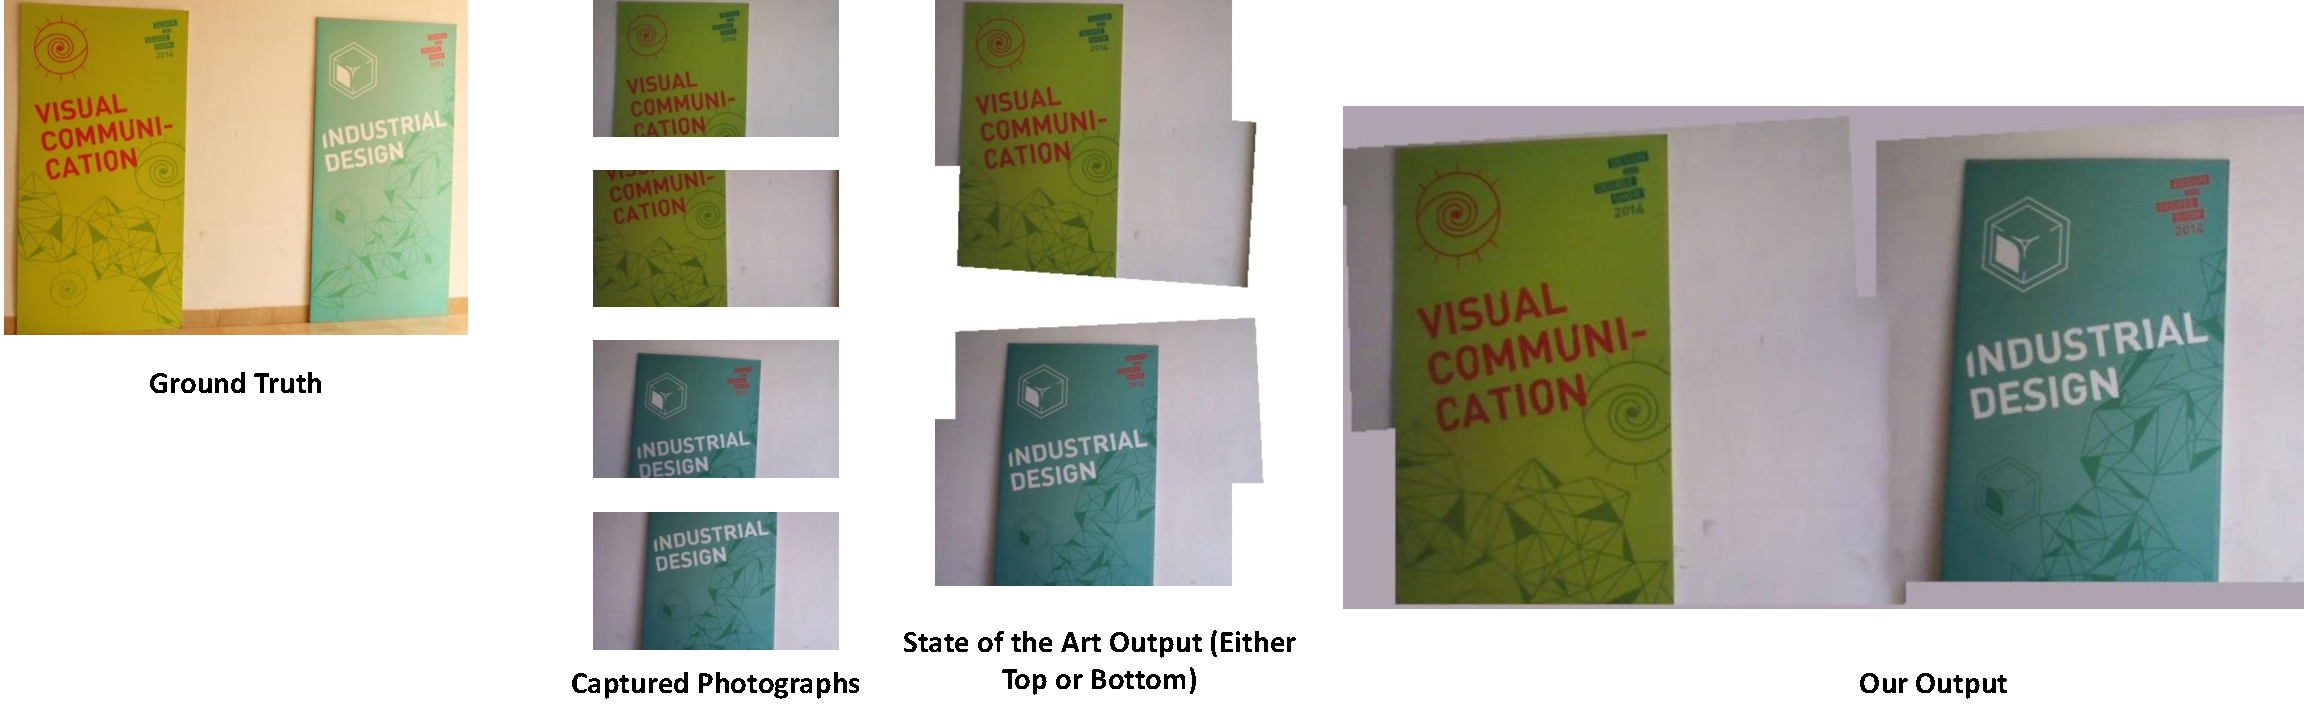
\includegraphics[width=0.49\textwidth]{figures/teaser2}
  \caption{ \label{fig:teaser} The ground truth picture shows a common
    situation in which dead space exists between large pictures (here,
    two poster boards). The input images (second column) show parts of
    the imagery obtained. Even if each of the images of the two
    individual posters can be stitched together (third column), the
    state of the art method encounter the dead space and is unable to
    make a complete mosaic.  It outputs either the first poster or the
    second, but not both together.  Our method (last column) succeeds
    since the acquired imagery is done using a quadcopter that has
    positional information.}
\end{figure}

{\bf Key Idea} We propose to solve the dead space problem by
using an inexpensive off-the-shelf flying device, such as a
quadcopter.  An autonomous programmed quadcopter is particularly
enticing because of its ability to fly to areas that are accessible to
the human eye, but inaccessible for the human to reach.  Such areas do not lend
themselves easily to high quality orthographic images. Our solution
uses coarse, approximate positional information that a quadcopter
can be assumed to have.  The proximity relationship that the resultant
images have can be used to significantly reduce the search space. 

{\bf Contributions} The main technical contributions of this paper is
that it improves the state of the art in mosaicing.  Sending a battery
of images from a quadcopter to an image stitching algorithm such as
Autostitch incapacitates the algorithm because of the sheer number of
images. Sending a sampled version of images to a manageable number $N$
of images, with $O(N^2)$ possible areas to match for features, also
does not work since the sampled image contains dead space.  In this
paper, we use positional information that lends itself to a graceful
$O(N)$ algorithm.  Some sample results are shown in Fig.\ 1 and Fig.\ 2.
Other results are available in the experiments section and also in the
supplementary material.

{\bf Challenges} In most stitching applications, both the scene and
the camera are stationary.  However when pictures are taken by a
flying quadcopter, virtually all relevant pictures that cover the
panaroma are taken from differing positions.  This makes the problem
harder than typical mosaicing problems.  In this paper, we assume that
the scene lies on a planar surface. The standard homography
computation is still not possible because the camera (the quadcopter)
is moving. We reduce the mosaicing problem to the stereo problem and
are thus able to complete the panaroma.

The rest of this paper is organized as follows.
\verb+TODO+

\section{Related Work}
\verb+TODO+

\section{Methodology}

The goal of this paper is to compute a panaroma of a scene lying on
one or many planar surfaces.  A schematic of two possible scenes for
this problem is shown in Fig.~\ref{fig:schematic}.

\begin{figure}[h!]
  \centering
  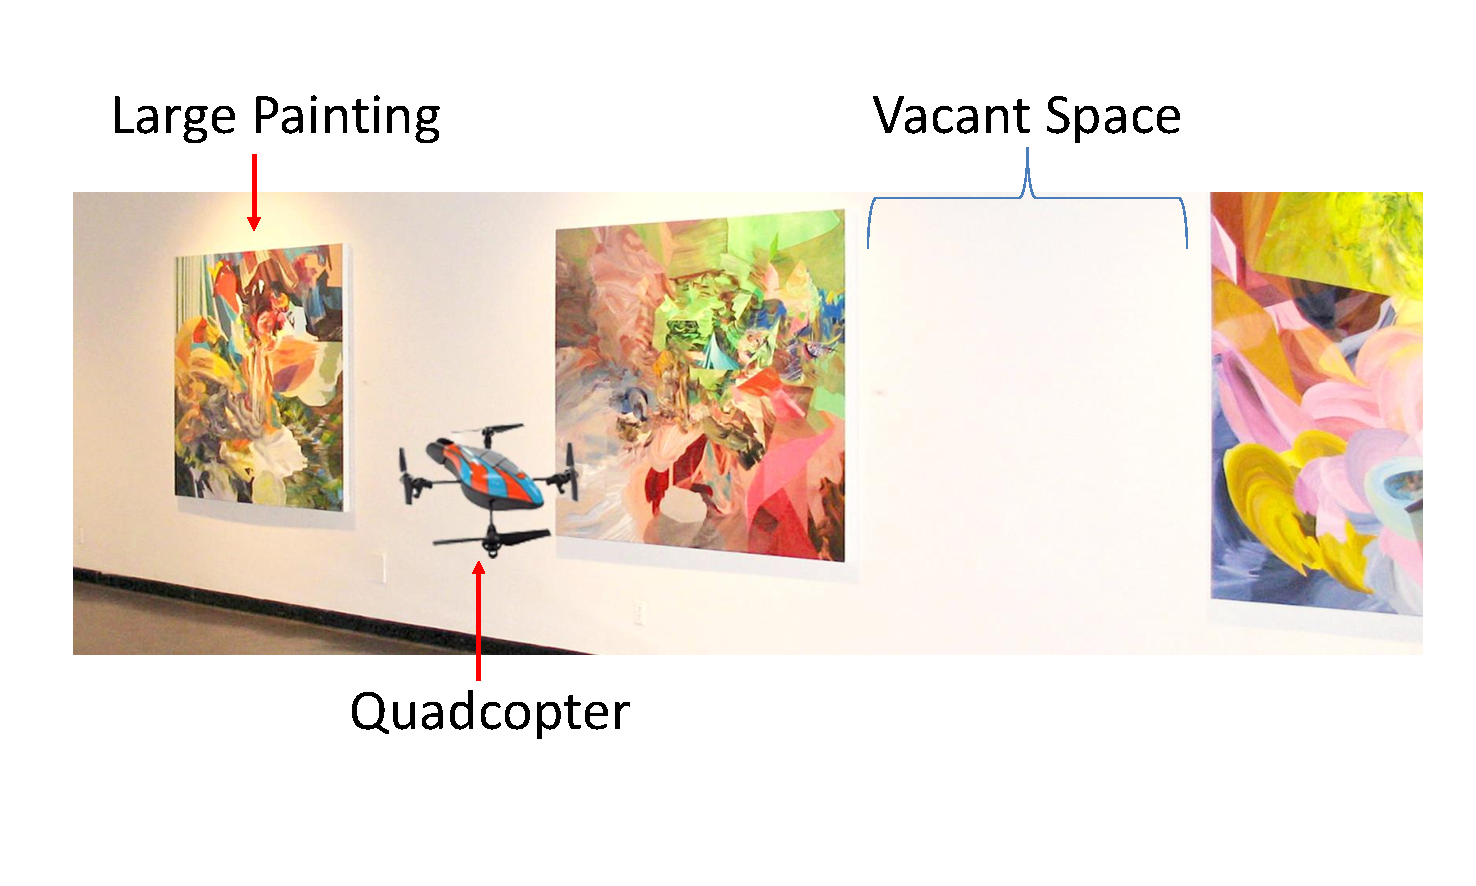
\includegraphics[width=0.49\textwidth]{figures/indoor} 
  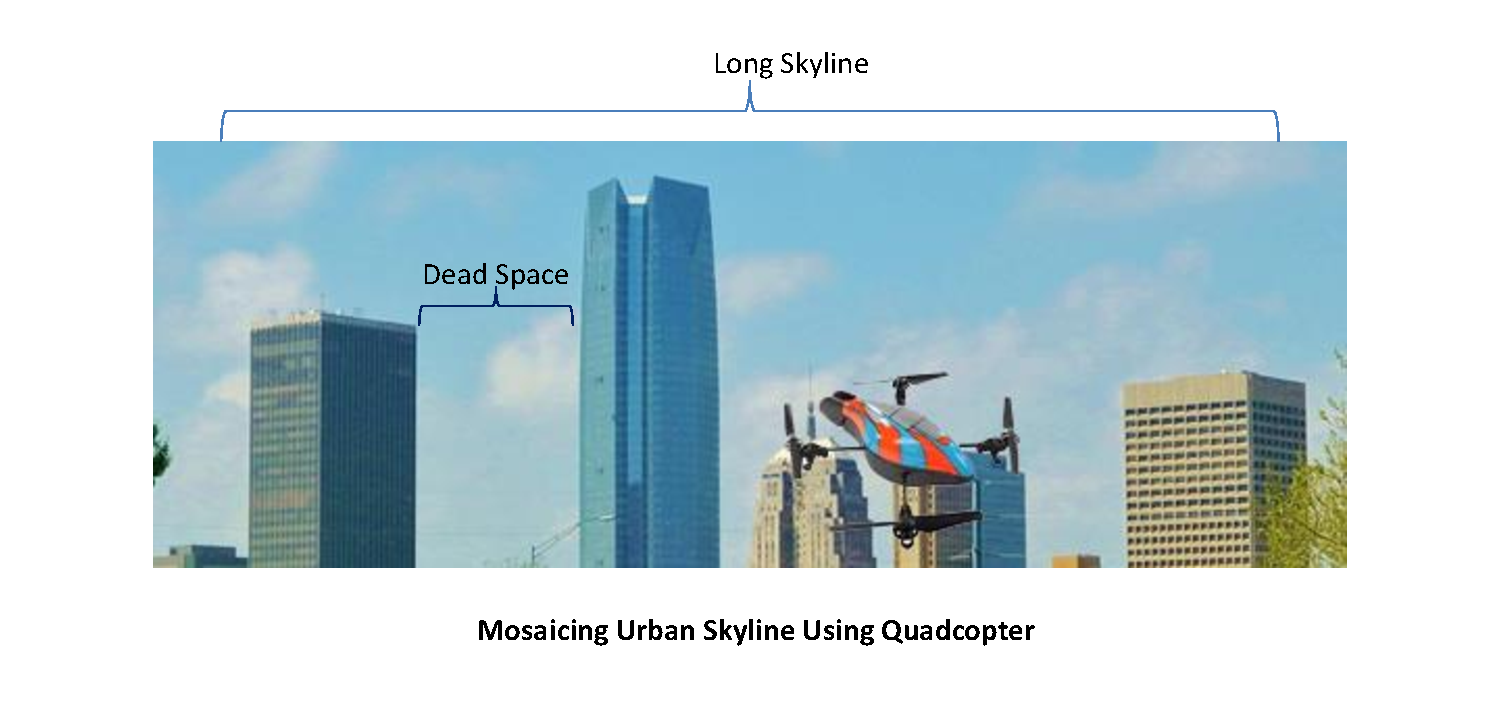
\includegraphics[width=0.49\textwidth]{figures/outdoor}
  \caption{ \label{fig:schematic} Dead space is
    encountered in both indoor and outdoor scenes.  When individual
    portions are captured by a quadcopter, how does one create the
    mosaic when features are not available?
  }
\end{figure}    


The method adopted consists of three steps described below. An
overview is shown in Fig.~\ref{fig:workflow}.

\begin{figure}[b!]
  \centering
  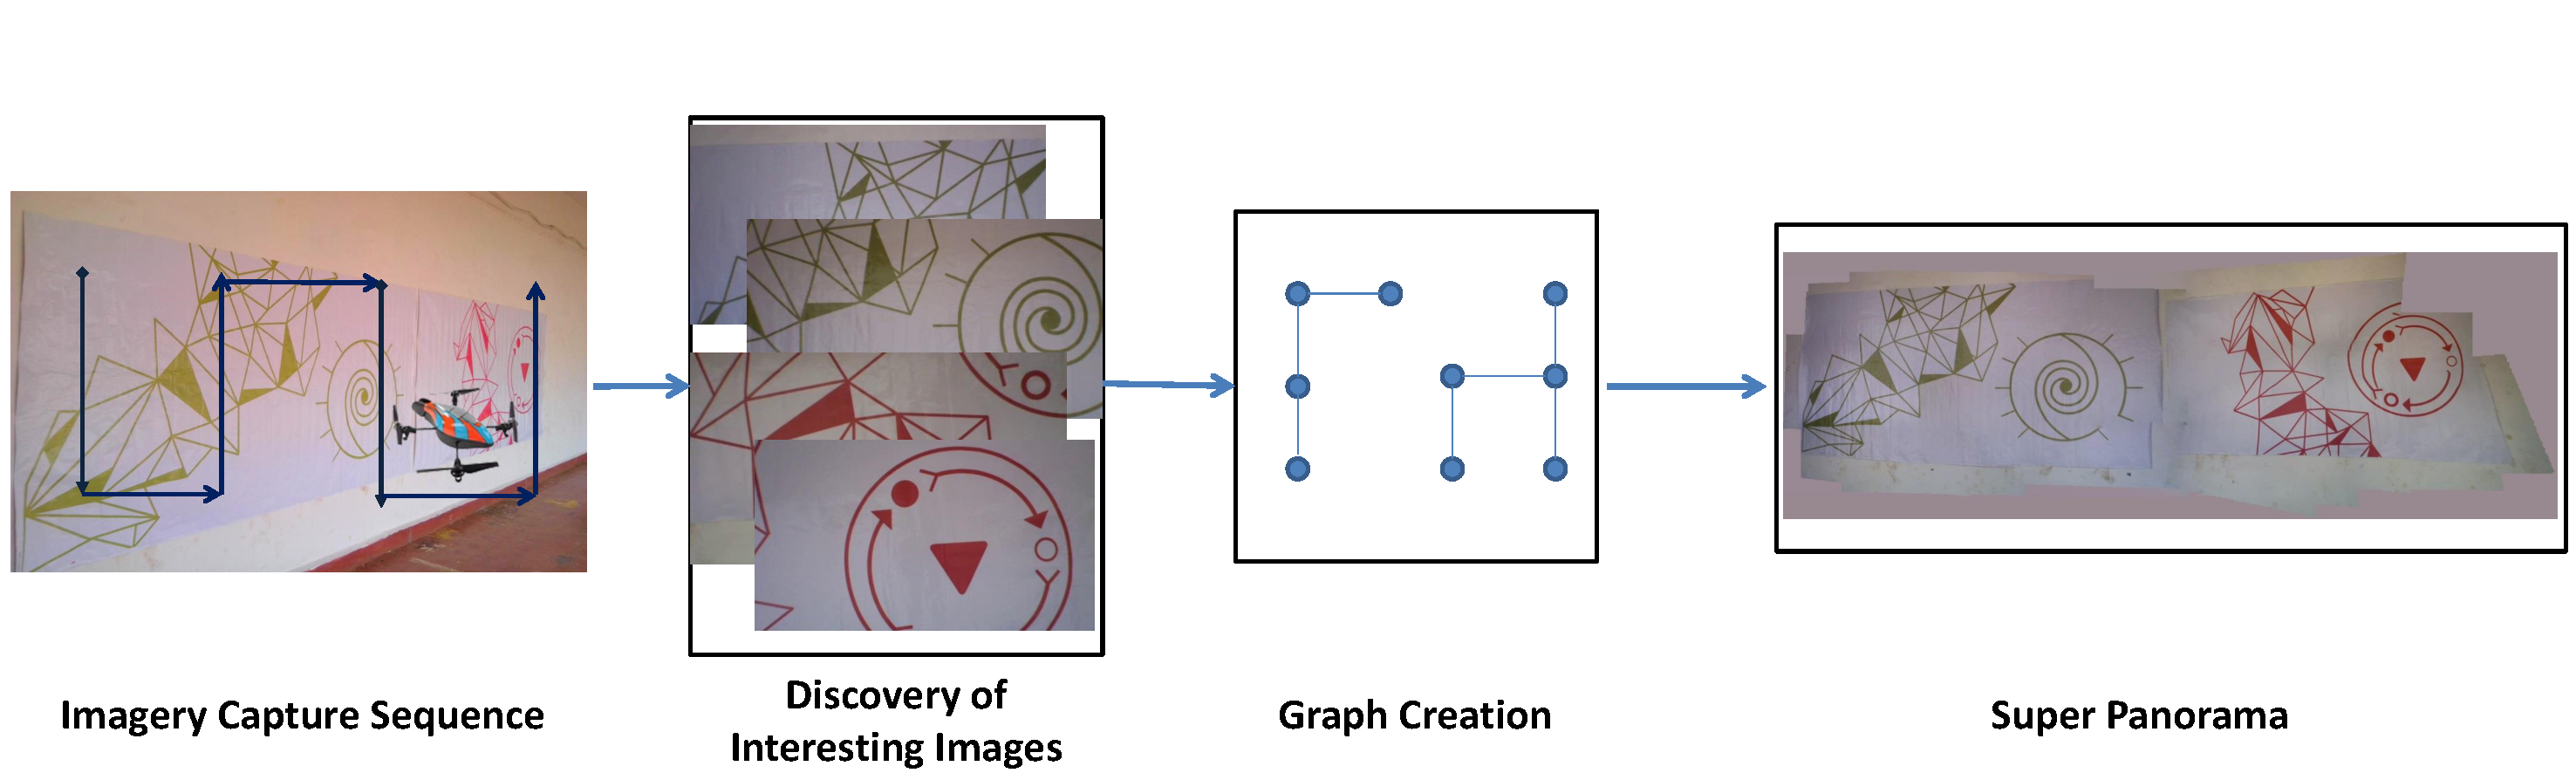
\includegraphics[width=0.49\textwidth]{figures/Workflow} 
  \caption{ \label{fig:workflow} Input imagery is acquired (column 1) by
    a quadcopter in a systematic fashion.  In the next step (column 2),
    interesting images are acquired by clustering the video into
    regions. A mosaic is constructed for each cluster.  A graph
    (column 3) is constructed, to facilitate a super panaroma (last
    column). Each step is described in more detail in this section.
  }
\end{figure}    


\begin{enumerate}
\item We first despatch the quadcopter to as close to the scene as
  possible. The corners of a rectangular area is provided to the
  quadcopter, and it is programmed to traverse the area in a snake
  like raster scan fashion.  There are various control aspects
  involved in sending a quadcopter; in outdoor areas, the quadcopter
  is impacted by wind and it might lose its way.  The control aspects
  of the quadcopter is beyond the scope of this paper.

  The quadcopter returns with a video of the scene.  Any short video
  of about a minute or more when given to a stitching program such as
  Autostitch overwhelms the progams rendering it unusable. In the rest
  of this section, we use Autostitch to indicate state of the art
  stitching programs such as Autostitch, Photoshop, etc.

\item Our goal in this step is to reduce the amount of data and
  produce a set of interesting images.  In other words, we wish to
  convert a video into an album of images.  We employ fairly standard
  methods available in the literature.  For each frame, we compute
  a set of global image descriptors such as color histogram, edges,
  and so on, and run a clustering algorithm.  The number of cluster
  centers is generally determined by the deemed capacity of a
  stitching algorithm such as Autostitch. 

  The key difference between our problem and standard albumization is
  the use of approximate positional information.  A standard
  quadcopter has an Inertial Measurement Unit (IMU) that, after
  calibration, can give an approximate information of positions.  It
  is to be noted that this information can be quite incorrect.
  However the mix of positional information and image features is
  often sufficient to produce the necessary subset of `interesting
  images' which may now given as input to Autostitch.

  As mentioned in the introduction, as long as there are sufficiently
  varying and ``matchable'' features, Autostitch is able to perform a
  pleasant stitching.  However, if the features are in the ``wrong''
  positions, then the output is not acceptable. 

  Significantly, Autostitch has not been designed to use positional
  information. As a result if there are N input images, the program
  has to consider possible matches in an $O(N^2)$ set of areas.  Our
  program is able to mosaic in an $O(N)$ fashion. 
 
  Specifically, we assume at this point that the interesting photos
  are available in the form of a $m \times n$ grid. We create a graph
  with images being nodes and postulate edges between two nodes if we
  are able to ``do successful matches''. Recall at this point that if
  there are ``dead spaces'' there will not be enough features for
  successful matches; the graph will end up with multiple
  (disconnected) components.  We next compute multiple spanning trees
  for the various components. If the result is single tree, then we
  stitch all pictures using the homographies.  The spanning tree is an
  $O(N)$ structure. 


\item In the previous step, Autostitch assumes that the input depth of
  the camera from the scene is the same. However, this is often not
  the case for at least two reasons.

  First, it is invariably difficult if not impossible to control a
  quadcopter to be at the exact depth even in indoor scenes.  The aero
  dynamics and the thrust produced tends to make the quadcopter drift.
  Second, it might also be necessary to let the quadcopter probe
  closer to the scene so as to get a ``good picture''.

  We assume that the output of the previous step has resulted in
  multiple spanning trees where each cluster center corresponds to a
  specific depth. We now create individual panoramas for each spanning
  tree and proceed to create a super-panorama.  

  A super panaroma is done using a two step process. Assume two trees
  in the forest corresponding to area X and area Y of the
  scene. Assume that depth of the planar surface is more for X than
  for Y. We then take the (panaromic) image captured at Y, and move it
  to a new location Y’ whose depth (from the imaged wall) is the same
  as that of X. (The resulting image Y’ will be smaller than Y). We
  can now think of these two images X and Y’ forming a stereo pair, so
  using the stereo disparity formula we can ``place'' Y’ from the view
  point of X.

\end{enumerate}



\section{Experiments and Results}

All our experiments have been completed with the inexpensive consumer
drone AR Parrot

{\color{red} Give details of this drone.}

The computing environment used was: (May not be necessary to talk
about TUM software?)

For the purposes of establishing the ground truth, pictures were taken
with a Canon ....


\subsection{Establishing Correctness}

In our first experiment, we wanted to ensure that the selection of
images done was comprehensive.  This experiment was conducted in an
outdoor environment.  Fig. x  shows examples of selected
images.  The video is available in the supplementary material.

\begin{verbatim}
https://drive.google.com/folderview?id=0ByIBGTG2uWf1flhxX1dNTHg5OUpxdVBYVnRHXzQtUndNWDREdWVhMTAzRk9aMVR0WnZlV3c&usp=sharing
\end{verbatim}
We note here that there were approximately 9000 images in the raw
video.  Autostitch was unable to cope when fed with 

Our selection algorithm was employed and approximately N=?? images
were obtained.  These were then fed to both Autostitch and the
stitching portion of our algorithm.  The results are shown in Fig. x1
and Fig x2.

\begin{verbatim}
https://drive.google.com/folderview?id=0ByIBGTG2uWf1fjZpNzJoVG1vYVNNZXhZSjNQaTh1OTlCMmNzak02Vk4xQVUta0hXaU43bUE&usp=sharing
\end{verbatim}

{\color{red} Say something about our stitching algorithm here?
  Anything noteworthy?}

\begin{verbatim}
https://drive.google.com/folderview?id=0ByIBGTG2uWf1fnExX3A5WUt3WkJIM1JzU0VvTTdpdTFOeVl6aWVFTHM2TUpKVXN2V1ZoYm8&usp=drive_web
\end{verbatim}

\subsection{Indoor Imagery with Dead Space} 

Our next selection of experiments were conducted in an indoor
environment with some natural light.  The input stream had about 4300
images.  

A sample of the images are available at

\begin{verbatim}
https://drive.google.com/folderview?id=0ByIBGTG2uWf1fjhjbkdyOW9odWxzYmE2V2FfaWtLRDBxeUtyNFFUbnFEV2hYeWRvY0w1enc&usp=sharing
\end{verbatim}

The selection algorithm pruned the video into N=?? images.
There were two  disconnected components in the resulting graph.  

The ground truth can be seen at

\begin{verbatim}
https://docs.google.com/file/d/0ByIBGTG2uWf1eU5LMVQzZmtqQnM/edit
\end{verbatim}

The resulting output can be seen at 

\begin{verbatim}
https://drive.google.com/file/d/0ByIBGTG2uWf1ZHpmNENZWGF4bkU/view
\end{verbatim}

One can see a better orthographic view of the posters in a composite
manner. 

Autostitch was unable to produce any reasonable output.


\subsection{Outdoor Imagery with Dead Space}

{\color{red} Not sure where the data is but we need a format similar
  to the above.}

\section{Concluding remarks}

In this paper, we have defined a new problem, that of computing a
mosaic of a planar scene with dead space.  Dead space relates to images
in an input stream where there are not enough features for traditional
mosaicing algorithms to stitch together a pleasing composite.  

Our solution to this problem is to use an autonomous quadcopter which
is capable of taking pictures.  The quadcopter has an inertial
measurement unit that is capable of outputting approximate
positions. Using this positional information, our algorithm selects an
``interesting'' subset of the video imagery.  This subset consists of
pictures taken with a ``moving'' camera; we reduce the resulting
problem of computing a mosaic by reduction to the stereo problem.  Our
method works on both indoor and outdoor scenes.

{\bf Future work} Controlling a consumer-focused inexpensive
quadcopter can be problematic; for instance the quadcopter could have
severe yaw and roll.  Vision based algorithms to control such
quadcopters might be quite useful.

\end{document}
